\chapter{Tinjauan Pustaka}
Tinjauan pustaka memuat teori, konsep, model, metode, atau sistem dari pustaka
ilmiah yang berkaitan dengan masalah penelitian, serta posisi penelitian ini
terhadap penelitian terdahulu.

\section{Penelitian Terdahulu}
Ringkas penelitian terdahulu yang relevan dan tunjukkan persamaan serta
perbedaannya dengan penelitian ini, seperti pada Tabel~\ref{tab:terdahulu}.

\begin{table}[htbp]
  \caption{Perbandingan penelitian terdahulu}
  \label{tab:terdahulu}
  \centering
  \begin{tabular}{|c|p{0.3\textwidth}|p{0.22\textwidth}|p{0.25\textwidth}|}
    \hline
    \textbf{No} & \textbf{Penelitian} & \textbf{Metode} & \textbf{Perbedaan} \\
    \hline
    1 & LeCun dkk. \cite{lecun1998gradient} & CNN & Objek data berbeda \\
    \hline
    2 & Vaswani dkk. \cite{vaswani2017attention} & Transformer & Domain tugas berbeda \\
    \hline
  \end{tabular}
  \sumber{\cite{lecun1998gradient,vaswani2017attention}}
\end{table}

\section{Landasan Teori}
Jelaskan teori yang dipakai dalam penelitian. Subbab berikut mencontohkan
penulisan persamaan, gambar, dan kode sumber.

\subsection{Persamaan}
Persamaan diberi nomor berdasarkan bab dan urutan kemunculannya, lalu diacu
sebagai Persamaan~\ref{eq:bobot}.
\begin{equation}
  V_i = \sum_{j=1}^{n} W_j \, r_{ij}
  \label{eq:bobot}
\end{equation}
Gunakan simbol yang tepat, misalnya $3 \times 4$, bukan huruf x.

\subsection{Gambar}
Judul gambar diletakkan di bawah gambar, seperti pada Gambar~\ref{fig:arsitektur}.
\begin{figure}[htbp]
  \centering
  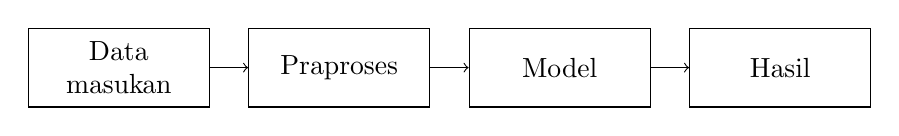
\begin{tikzpicture}[node distance=2.8cm,
      kotak/.style={draw, minimum width=2.3cm, minimum height=1cm, align=center}]
    \node[kotak] (masukan) {Data\\masukan};
    \node[kotak, right of=masukan] (proses) {Praproses};
    \node[kotak, right of=proses] (model) {Model};
    \node[kotak, right of=model] (keluaran) {Hasil};
    \draw[->] (masukan) -- (proses);
    \draw[->] (proses) -- (model);
    \draw[->] (model) -- (keluaran);
  \end{tikzpicture}
  \caption{Arsitektur umum sistem}
  \label{fig:arsitektur}
\end{figure}

Gambar dari sumber lain wajib disertai sitasi di bawahnya dan dicantumkan di
daftar pustaka \cite{goodfellow2016deep}.

\subsection{Kode Sumber}
Kode sumber hanya dituliskan jika benar-benar diperlukan. Pedoman mensyaratkan
Courier New 9 pt, spasi tunggal, dan nomor baris.
\begin{lstlisting}[caption={Fungsi iteratif}]
def jumlah(data):
    total = 0
    for nilai in data:
        total += nilai
    return total
\end{lstlisting}
